\FloatBarrier
\begin{figure}[!h]
\centering
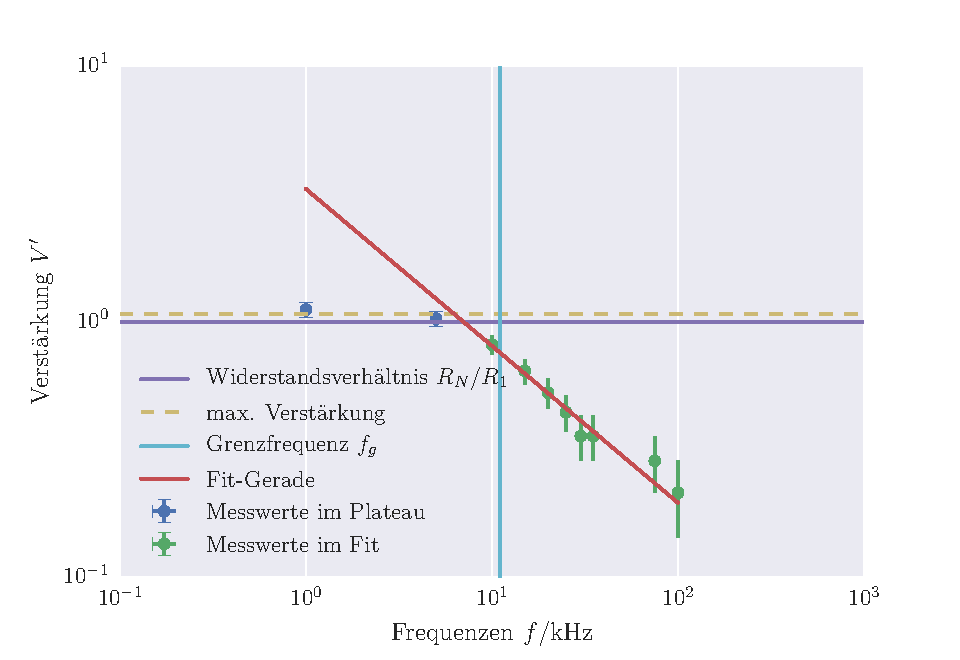
\includegraphics[scale=1]{../Grafiken/Gegengekoppelter_Verstaerker_1.pdf}
\caption{Doppellogarithmische Darstellung der Verstärkung der ersten gegengekoppelten Verstärkerschaltung in Abhängigkeit der Frequenz der Eingangsspannug. Zusätzlich wurden die Ausgleichsgerade
	durch die abfallenden Messwerte und eine senkrechte Gerade bei der Grenzfrequenz eingezeichnet. Ferner sind noch  zwei waagerechte Geraden dargestellt. Die eine markiert den Mittelwert der Messwerte im Plateau und die  andere
	den theoretischen Wert dieser Größe.
	\label{fig:gegengekoppelter_verstaerker_1}}
\end{figure}
\FloatBarrier